\documentclass[11pt,a4paper]{article}
\usepackage[utf8]{inputenc}
\usepackage[T1]{fontenc}
\usepackage[brazil]{babel}
\usepackage{lmodern}
\usepackage[margin=2cm]{geometry}
\usepackage{amsmath,amssymb}
\usepackage{booktabs}
\usepackage{graphicx}
\usepackage{xcolor}
\usepackage{titlesec}
\usepackage{tabularx}
\usepackage[section]{placeins}
\usepackage{float}
\usepackage{hyperref}

\graphicspath{{../results/figures/}}

\hypersetup{
    colorlinks=true,
    linkcolor=blue!70!black,
    citecolor=blue!70!black,
    urlcolor=blue!70!black
}

\titleformat{\section}{\large\bfseries}{\thesection.}{0.5em}{}
\titleformat{\subsection}{\normalsize\bfseries}{\thesubsection.}{0.5em}{}
\titlespacing*{\section}{0pt}{1.2ex plus 0.5ex minus .2ex}{0.6ex}
\titlespacing*{\subsection}{0pt}{1.0ex plus 0.4ex minus .2ex}{0.4ex}

\setlength{\parskip}{0.45em}
\setlength{\parindent}{0pt}

\begin{document}

\begin{center}
    {\LARGE \textbf{Projeto 3: Modelos Generativos}} \\[0.3em]
    {\large Autoencoder Variacional (VAE) no Fashion-MNIST} \\[0.3em]
    {\large Disciplina: Introdução às Redes Neurais Artificiais} \\[0.3em]
    \textbf{Autor:} Arthur Santos de Oliveira (RA: 156297) \\[0.2em]
    \textbf{Repositório / Código Reprodutível:} \url{https://github.com/Arthur-so/introducao-a-redes-neurais}
\end{center}
\vspace{-0.5em}
\hrule
\vspace{0.8em}

\section{Configuração Experimental}

\subsection{Dados e Partição}

O Fashion-MNIST tem 70.000 imagens de roupas e acessórios em tons de cinza, com $28\times28$ pixels, divididas em 10 classes: camiseta, calça, suéter, vestido, casaco, sandália, camisa, tênis, bolsa e bota. Cada imagem foi achatada num vetor de 784 pixels, e cada pixel foi dividido por 255 para ficar em $[0, 1]$. A partição usada foi:
\begin{itemize}
    \item \textbf{Treino:} 50.000 imagens, sorteadas das 60.000 de treino do conjunto original;
    \item \textbf{Validação:} as outras 10.000 imagens de treino, usadas para escolher a topologia;
    \item \textbf{Teste:} as 10.000 imagens de teste originais, usadas só na avaliação final e nos gráficos do espaço latente.
\end{itemize}
Os rótulos não são usados no treino. Eles servem apenas para pintar os pontos nos gráficos do espaço latente.

\subsection{Modelo e Função de Custo}

O VAE tem duas redes MLP. O \textbf{codificador} recebe a imagem $x$ e devolve a média $\mu_x$ e o desvio padrão $\sigma_x$ de uma distribuição normal no espaço latente; na prática, a rede devolve $\log \sigma_x^2$, que pode assumir qualquer valor real. Um ponto é sorteado dessa distribuição pelo \textbf{truque de reparametrização}, $z = \mu_x + \sigma_x \zeta$, com $\zeta \sim N(0, I)$, e o \textbf{decodificador} reconstrói a imagem $d(z)$ a partir dele. A saída do decodificador passa por uma sigmoide, para ficar em $[0, 1]$, como os pixels.

A função de custo de cada imagem é a soma de dois termos:
\[
\text{custo} = \underbrace{\|x - d(z)\|^2}_{\text{reconstrução}} + \underbrace{KL\big(N(\mu_x, \sigma_x), N(0, I)\big)}_{\text{regularização}},
\qquad
KL = -\frac{1}{2}\sum_{j=1}^{k}\left(1 + \log\sigma_j^2 - \mu_j^2 - \sigma_j^2\right),
\]
em que a reconstrução soma o erro quadrático dos 784 pixels e $k$ é a dimensão do espaço latente. O custo de um conjunto é a média do custo das suas imagens. O termo KL puxa a distribuição de cada imagem para perto da normal padrão $N(0, I)$, o que mantém o espaço latente contínuo e permite gerar imagens novas sorteando $z \sim N(0, I)$.

\subsection{Hiperparâmetros e Busca da Topologia}

Para cada dimensão latente (2 e 8), foram treinadas 5 topologias, variando o número de camadas ocultas (1, 2 ou 3) e a largura (256 ou 512 neurônios na primeira camada). O decodificador usa as mesmas camadas do codificador, em ordem inversa. A topologia escolhida para cada dimensão foi a de \textbf{menor custo na validação}. Os demais hiperparâmetros ficaram fixos, com valores mais utilizados (Tabela~\ref{tab:hiper}).

\begin{table}[H]
\centering
\small
\caption{Espaço de busca e hiperparâmetros fixos.}
\label{tab:hiper}
\begin{tabularx}{\textwidth}{lX}
\toprule
\textbf{Item} & \textbf{Valor} \\
\midrule
Topologias do codificador & 784-256; 784-512; 784-256-128; 784-512-256; 784-512-256-128 \\
Dimensão latente & 2 e 8 (busca feita separadamente para cada uma) \\
Ativação & ReLU nas camadas ocultas; sigmoide na saída do decodificador \\
Otimizador & Adam, taxa de aprendizado $10^{-3}$ \\
Tamanho do lote & 128 \\
Épocas & 30; ficam os pesos da época de menor custo na validação \\
Semente & 42 \\
\bottomrule
\end{tabularx}
\end{table}

\section{Escolha da Topologia}

A Tabela~\ref{tab:busca} traz o custo na validação de cada topologia, na sua melhor época, separado nos dois termos. A Figura~\ref{fig:busca} mostra o custo na validação ao longo das épocas.

\begin{table}[H]
\centering
\small
\caption{Busca da topologia: custo na validação na melhor época (menor é melhor). Em negrito, a topologia escolhida para cada dimensão latente.}
\label{tab:busca}
\begin{tabular}{llrcccc}
\toprule
\textbf{Latente} & \textbf{Codificador} & \textbf{Parâmetros} & \textbf{Melhor época} & \textbf{Custo} & \textbf{Reconstrução} & \textbf{KL} \\
\midrule
2D & 784-256          & 404.244   & 30 & 28,03 & 23,18 & 4,85 \\
2D & 784-512          & 807.700   & 30 & 27,86 & 23,09 & 4,77 \\
2D & 784-256-128      & 469.268   & 30 & 26,24 & 21,10 & 5,14 \\
2D & 784-512-256      & 1.068.820 & 28 & 25,91 & 20,59 & 5,32 \\
\textbf{2D} & \textbf{784-512-256-128} & \textbf{1.133.844} & \textbf{21} & \textbf{25,86} & \textbf{20,77} & \textbf{5,10} \\
\midrule
8D & 784-256          & 408.864   & 29 & 24,33 & 15,80 & 8,54 \\
8D & 784-512          & 816.928   & 30 & 23,97 & 15,66 & 8,31 \\
8D & 784-256-128      & 471.584   & 26 & 23,74 & 16,90 & 6,83 \\
\textbf{8D} & \textbf{784-512-256} & \textbf{1.073.440} & \textbf{30} & \textbf{23,38} & \textbf{16,27} & \textbf{7,10} \\
8D & 784-512-256-128  & 1.136.160 & 30 & 23,83 & 17,59 & 6,24 \\
\bottomrule
\end{tabular}
\end{table}

\begin{figure}[H]
\centering
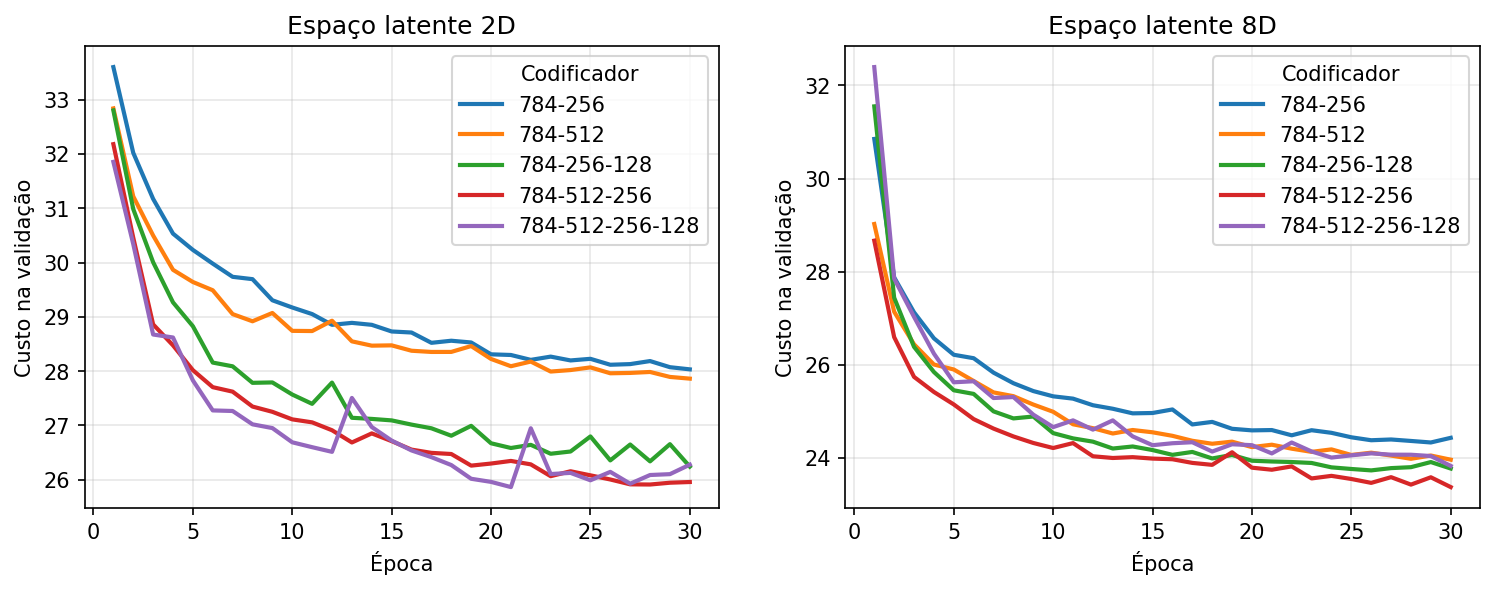
\includegraphics[width=\textwidth]{busca_topologia.png}
\caption{Custo na validação por época de cada topologia. Esquerda: espaço latente 2D; direita: 8D.}
\label{fig:busca}
\end{figure}

\begin{itemize}
    \item \textbf{Topologias escolhidas.} No espaço 2D, a melhor foi a de 3 camadas (784-512-256-128, custo 25,86); no 8D, a de 2 camadas (784-512-256, custo 23,38). No 2D, a diferença para a segunda colocada (784-512-256, 25,91) é de apenas 0,05, um empate na prática.
    \item \textbf{Profundidade pesou mais que largura.} No 2D, passar de 1 para 2 camadas reduziu o custo em cerca de 1,8 (de 28,03 para 26,24 com 256 neurônios), enquanto dobrar a largura da rede de 1 camada (de 256 para 512) reduziu só 0,17. No 8D, as diferenças entre topologias foram menores (de 23,38 a 24,33), e a rede de 3 camadas ficou atrás da de 2.
    \item \textbf{8D teve custo menor que 2D em todas as topologias.} A diferença está na reconstrução: entre 15,66 e 17,59 no 8D, contra 20,59 a 23,18 no 2D. Em compensação, o KL é maior no 8D (6,24 a 8,54, contra 4,77 a 5,32).
\end{itemize}

\textbf{Por quê.} Com 8 dimensões, o codificador pode guardar mais informação sobre cada imagem, e o decodificador a reconstrói melhor. Cada dimensão que se afasta de $N(0, 1)$ aumenta o termo KL, então o ganho na reconstrução vem com um KL maior. Com 2 dimensões, a rede precisa comprimir muito a imagem, e camadas a mais ajudam a fazer essa compressão.

A Figura~\ref{fig:treino_val} mostra as curvas de treino e validação dos dois modelos escolhidos.

\begin{figure}[H]
\centering
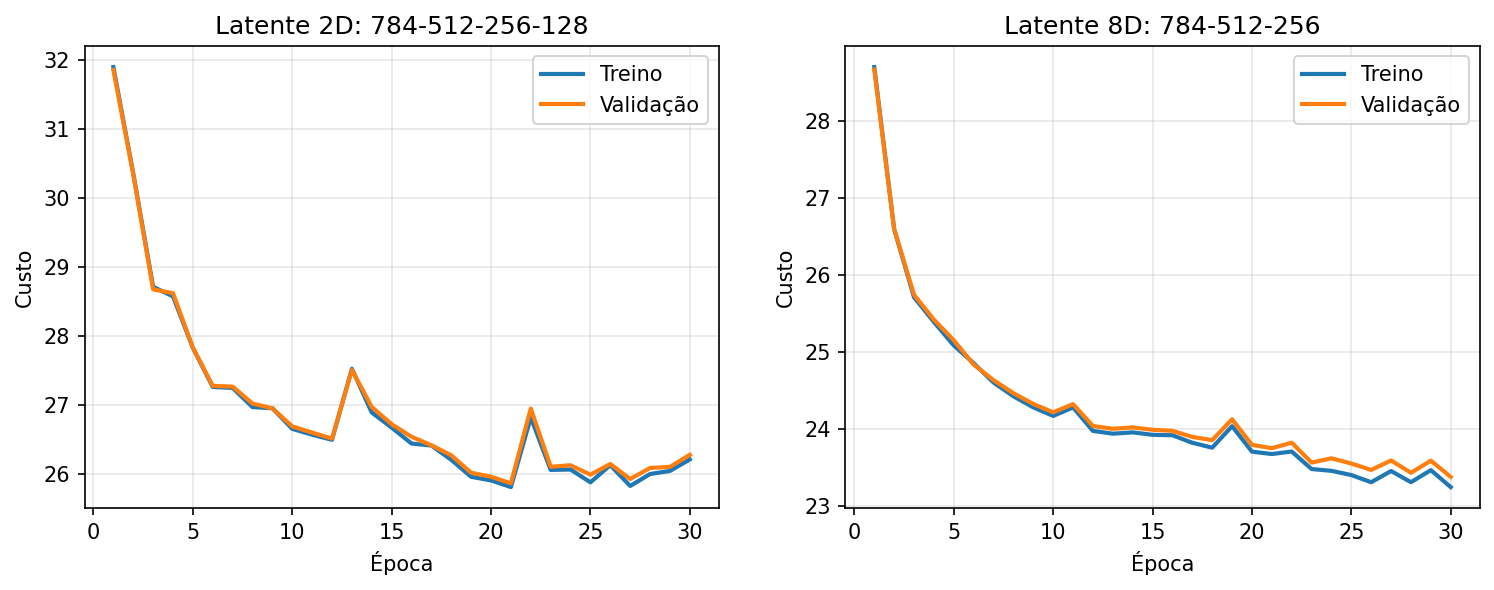
\includegraphics[width=\textwidth]{treino_validacao.png}
\caption{Custo de treino e de validação por época dos modelos escolhidos.}
\label{fig:treino_val}
\end{figure}

\begin{itemize}
    \item \textbf{Não houve sobreajuste.} As curvas de treino e validação ficam praticamente sobrepostas nos dois modelos durante as 30 épocas.
    \item \textbf{Picos no modelo 2D.} O modelo de 3 camadas teve dois saltos no custo (épocas 13 e 22), dos quais se recuperou nas épocas seguintes. Por isso a sua melhor época foi a 21, e não a última.
    \item \textbf{O custo ainda caía na época 30.} Na maioria das topologias, a melhor época ficou entre a 28 e a 30 (Tabela~\ref{tab:busca}). Mais épocas provavelmente reduziriam um pouco o custo, mas a comparação entre topologias foi feita com o mesmo número de épocas para todas.
\end{itemize}

\textbf{Conjunto de teste.} A Tabela~\ref{tab:teste} mostra o custo dos modelos escolhidos no teste. Os valores ficaram próximos dos da validação (25,86 e 23,38), o que confirma que não houve sobreajuste.

\begin{table}[H]
\centering
\small
\caption{Custo dos modelos escolhidos no conjunto de teste.}
\label{tab:teste}
\begin{tabular}{llccc}
\toprule
\textbf{Latente} & \textbf{Codificador} & \textbf{Custo} & \textbf{Reconstrução} & \textbf{KL} \\
\midrule
2D & 784-512-256-128 & 25,98 & 20,90 & 5,08 \\
8D & 784-512-256     & 23,52 & 16,45 & 7,07 \\
\bottomrule
\end{tabular}
\end{table}

\section{Reconstrução e Geração de Imagens}

A Figura~\ref{fig:reconstrucoes} mostra a primeira imagem de cada classe do conjunto de teste e a sua reconstrução pelos dois modelos (decodificando a média $\mu_x$).

\begin{figure}[H]
\centering
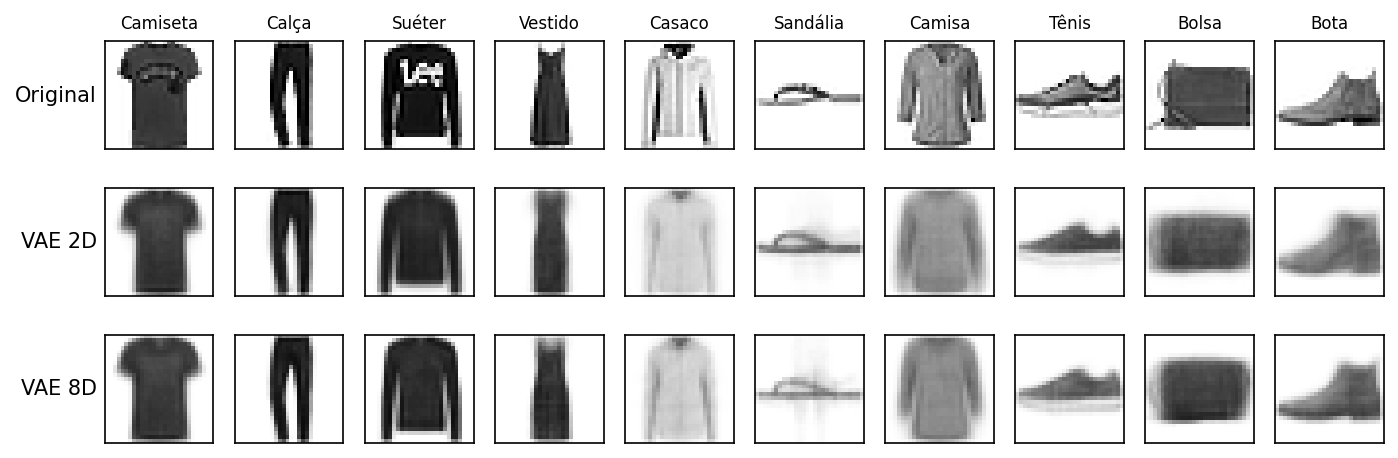
\includegraphics[width=\textwidth]{reconstrucoes.png}
\caption{Uma imagem de teste de cada classe (linha de cima) e as reconstruções dos VAEs 2D e 8D.}
\label{fig:reconstrucoes}
\end{figure}

Os dois modelos reconstroem a \textbf{forma e o tom geral} de todas as peças, mas as imagens ficam borradas e perdem detalhes finos: a estampa da camiseta, as letras do suéter, os detalhes do casaco e a alça da bolsa. A diferença visual entre 2D e 8D é pequena nesses exemplos, embora o erro de reconstrução no teste seja bem menor no 8D (16,45 contra 20,90).

A Figura~\ref{fig:amostras} mostra imagens \textbf{novas}, geradas decodificando 10 pontos sorteados de $N(0, I)$ em cada modelo.

\begin{figure}[H]
\centering
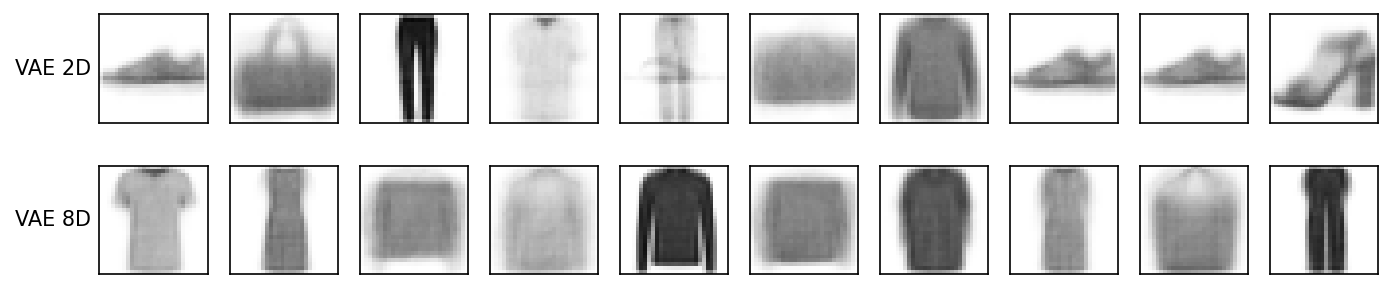
\includegraphics[width=\textwidth]{amostras_geradas.png}
\caption{Imagens geradas a partir de $z \sim N(0, I)$, sem usar nenhuma imagem de entrada.}
\label{fig:amostras}
\end{figure}

A maioria das imagens geradas é reconhecível como uma peça do conjunto: tênis, bolsas, calças, camisetas, suéteres e vestidos. A exceção é a 5ª imagem do modelo 2D, que mistura uma peça de roupa com uma sandália. Esse tipo de imagem aparece quando o ponto sorteado cai entre dois grupos do espaço latente (Seção~\ref{sec:latente2d}).

\section{Espaço Latente 2D}
\label{sec:latente2d}

A Figura~\ref{fig:latente2d} mostra a representação latente ($\mu_x$) das 10.000 imagens de teste no modelo 2D, com cada ponto pintado pela classe da imagem.

\begin{figure}[H]
\centering
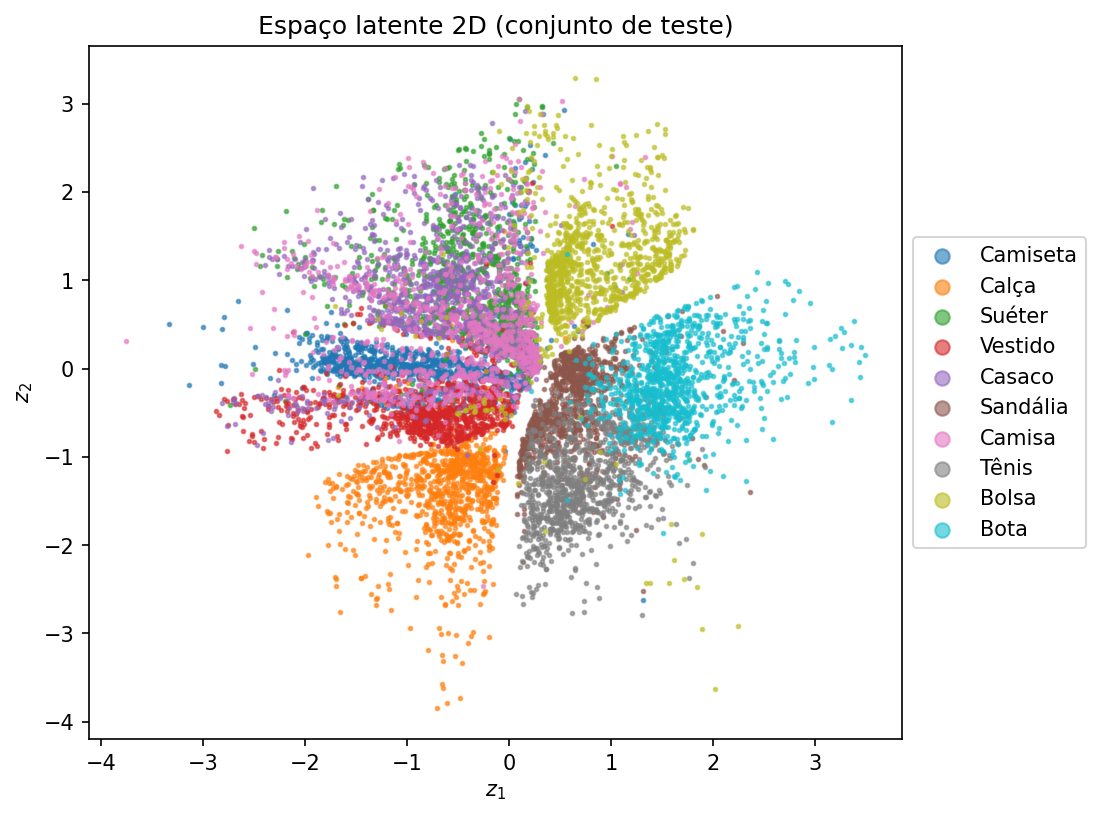
\includegraphics[width=0.75\textwidth]{espaco_latente_2d.png}
\caption{Espaço latente 2D: média $\mu_x$ de cada imagem de teste, pintada pelo rótulo.}
\label{fig:latente2d}
\end{figure}

\begin{itemize}
    \item \textbf{Há formação de clusters.} Os calçados (sandália, tênis e bota) ocupam a parte direita e inferior direita; as bolsas, a parte superior direita; as calças, a parte inferior esquerda; e as peças que cobrem o tronco (camiseta, suéter, casaco, camisa e vestido), a metade esquerda.
    \item \textbf{A separação dos rótulos depende da classe.} Calça, bolsa, bota e tênis formam grupos bem separados. A sandália fica entre o tênis e a bota, encostada nos dois. Camiseta e vestido formam faixas próprias, mas encostadas uma na outra. \textbf{Suéter, casaco e camisa ficam misturados} na parte superior esquerda.
    \item \textbf{Distribuição perto da normal padrão.} Quase todos os pontos ficam entre $-3$ e $3$ nos dois eixos, centrados na origem, como o termo KL incentiva.
\end{itemize}

\textbf{Por quê.} O VAE agrupa imagens parecidas, pois imagens próximas no espaço latente geram reconstruções parecidas. Suéter, casaco e camisa têm a mesma silhueta (tronco com manga comprida) e diferem em detalhes finos, que o modelo 2D não consegue representar (Figura~\ref{fig:reconstrucoes}). Por isso essas classes se sobrepõem. A calça, a bolsa e os calçados têm formas bem diferentes de todas as outras classes, e por isso ficam separados.

A Figura~\ref{fig:varredura} decodifica uma grade de $15\times15$ pontos do espaço latente, de $-3$ a $3$ em cada eixo. Cada imagem está na posição $(z_1, z_2)$ que a gerou, e a figura pode ser comparada diretamente com a Figura~\ref{fig:latente2d}.

\begin{figure}[H]
\centering
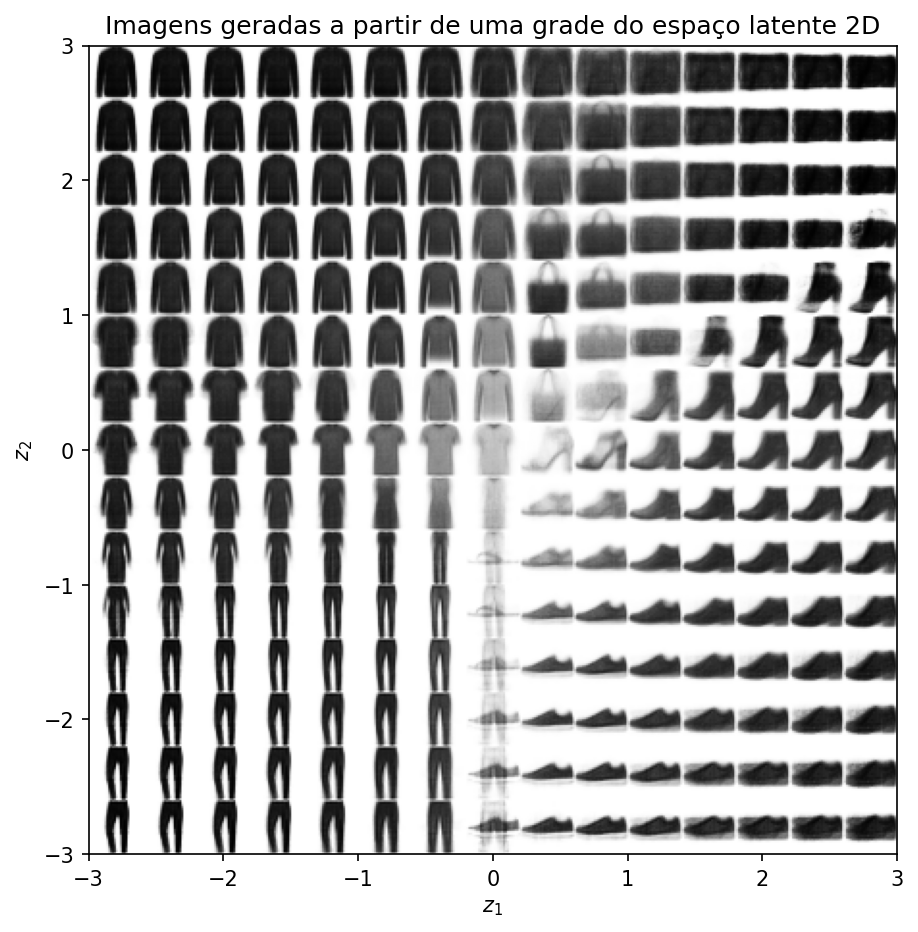
\includegraphics[width=0.65\textwidth]{varredura_latente_2d.png}
\caption{Imagens geradas pelo decodificador do modelo 2D numa grade de pontos do espaço latente.}
\label{fig:varredura}
\end{figure}

\begin{itemize}
    \item \textbf{As regiões batem com os clusters.} Peças de manga comprida no alto à esquerda, camisetas e vestidos no meio à esquerda, calças embaixo à esquerda, bolsas no alto à direita, botas no meio à direita e tênis embaixo à direita.
    \item \textbf{O espaço é contínuo.} As imagens mudam aos poucos entre pontos vizinhos: o suéter encurta a manga e vira camiseta, a camiseta afina e vira vestido, e a bota vira um sapato de salto e depois uma sandália.
    \item \textbf{Regiões entre grupos geram imagens misturadas.} Em $z_1 \approx 0$, abaixo de $z_2 = -1$, entre as calças e os tênis, as imagens são borradas e misturam as duas peças. Na Figura~\ref{fig:latente2d}, essa é uma faixa com poucas imagens de teste.
\end{itemize}

\section{Espaço Latente 8D Projetado com PCA}

Para visualizar o espaço 8D, a média $\mu_x$ das imagens de teste foi projetada nas duas primeiras componentes principais (PCA). A Figura~\ref{fig:pca} mostra a projeção com os rótulos, e a Figura~\ref{fig:variancia} mostra a fração da variância explicada por cada componente.

\begin{figure}[H]
\centering
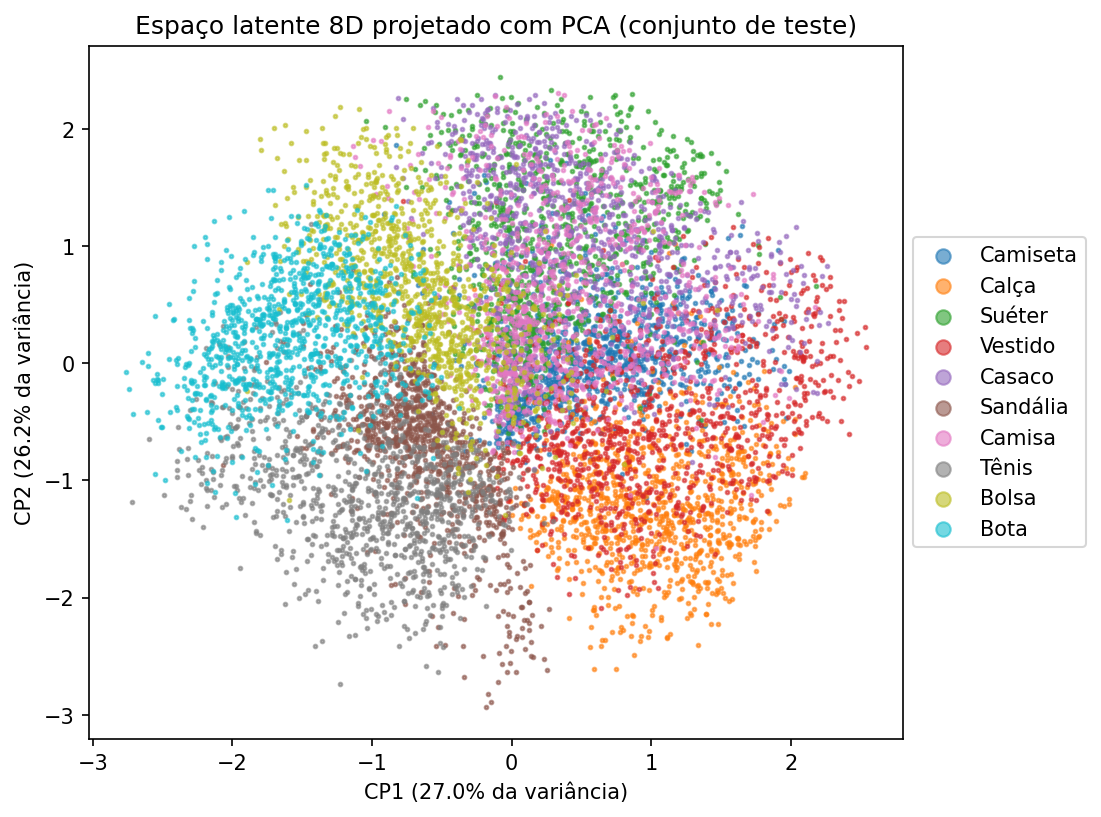
\includegraphics[width=0.75\textwidth]{espaco_latente_8d_pca.png}
\caption{Espaço latente 8D projetado nas duas primeiras componentes principais (CP1 e CP2), pintado pelo rótulo.}
\label{fig:pca}
\end{figure}

\begin{figure}[H]
\centering
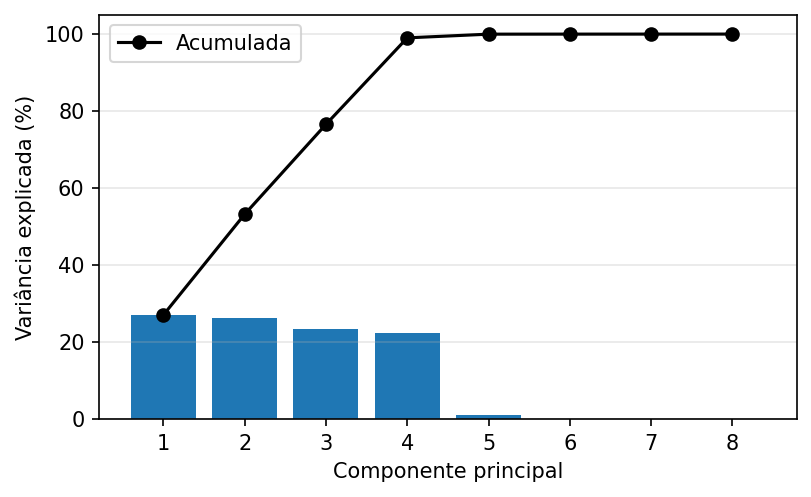
\includegraphics[width=0.6\textwidth]{variancia_pca_8d.png}
\caption{Variância explicada por cada componente principal do espaço latente 8D (barras) e acumulada (linha).}
\label{fig:variancia}
\end{figure}

\textbf{A projeção ilustra 53,2\% da variância}: 27,0\% na CP1 e 26,2\% na CP2. As componentes 3 e 4 explicam quase o mesmo (23,4\% e 22,5\%), e as quatro primeiras juntas chegam a 99,0\%. As componentes 5 a 8 somam menos de 1\%.

\textbf{Por que só 4 componentes importam.} O modelo 8D usa só 4 das suas 8 dimensões latentes (Tabela~\ref{tab:uso}). Nas dimensões 1, 3, 5 e 8, a média $\mu$ fica praticamente igual para todas as imagens (variância de no máximo 0,036) e o desvio $\sigma$ fica perto de 1, ou seja, a distribuição dessas dimensões é a própria $N(0, 1)$ e não carrega informação sobre a imagem. Como o termo KL cobra por cada dimensão que se afasta de $N(0, 1)$, o modelo só usa uma dimensão se ela melhorar a reconstrução o bastante, e 4 dimensões foram suficientes.

\begin{table}[H]
\centering
\small
\caption{Uso de cada dimensão do espaço latente 8D nas imagens de teste: variância de $\mu$ entre as imagens e $\sigma$ médio.}
\label{tab:uso}
\begin{tabular}{lcccccccc}
\toprule
\textbf{Dimensão} & 1 & 2 & 3 & 4 & 5 & 6 & 7 & 8 \\
\midrule
Variância de $\mu$ & 0,000 & 0,844 & 0,001 & 0,994 & 0,001 & 0,974 & 0,883 & 0,036 \\
$\sigma$ médio      & 0,999 & 0,267 & 0,988 & 0,124 & 1,001 & 0,121 & 0,276 & 0,975 \\
\bottomrule
\end{tabular}
\end{table}

\begin{itemize}
    \item \textbf{Há formação de clusters}, nas mesmas famílias do espaço 2D: calçados à esquerda (bota, sandália e tênis), bolsas acima deles, calças e vestidos embaixo à direita e as peças de tronco no alto, no centro.
    \item \textbf{A separação na projeção é menor que no espaço 2D.} Os grupos se encostam mais: bolsa toca a bota e as peças de tronco, vestido se mistura com calça e com camiseta, e camiseta, suéter, casaco e camisa se sobrepõem no centro.
    \item \textbf{Cuidado com a leitura.} A projeção mostra só 53,2\% da variância. Pontos que se sobrepõem na projeção podem estar separados nas componentes 3 e 4, que juntas têm outros 45,8\%. Já no modelo 2D, o gráfico mostra o espaço latente inteiro.
\end{itemize}

\section{Discussão e Conclusões}

\begin{itemize}
    \item \textbf{Há formação de clusters no espaço latente?} Sim, nos dois modelos. As imagens se agrupam por forma: calçados, bolsas, calças e peças de tronco ocupam regiões diferentes, mesmo sem os rótulos serem usados no treino.
    \item \textbf{Há separação dos rótulos?} Parcial. Calça, bolsa, bota e tênis ficam bem separados; sandália, camiseta e vestido ficam encostados nos grupos vizinhos; suéter, casaco e camisa se misturam, pois têm a mesma silhueta. A separação é mais clara no gráfico 2D do que na projeção do 8D.
    \item \textbf{Quanto da variância a projeção ilustra?} 53,2\% (27,0\% + 26,2\%). O modelo 8D usa apenas 4 dimensões, e as 4 primeiras componentes somam 99,0\% da variância.
    \item \textbf{2D vs.\ 8D.} O modelo 8D teve custo menor (23,52 contra 25,98 no teste), graças a uma reconstrução melhor, mas ainda assim usou só 4 das 8 dimensões. O modelo 2D reconstrói pior, mas o seu espaço latente pode ser visto por inteiro e percorrido diretamente (Figura~\ref{fig:varredura}).
    \item \textbf{Topologia.} Para o espaço 2D, redes mais profundas reduziram bem o custo; para o 8D, as diferenças entre topologias foram pequenas, e a rede de 2 camadas foi a melhor.
    \item \textbf{Limitações.} As imagens reconstruídas e geradas são borradas e sem detalhes finos. O custo ainda caía na época 30 em quase todas as topologias, e a diferença entre as duas melhores topologias do 2D (0,05) é pequena demais para apontar uma vencedora clara com uma única semente.
\end{itemize}

\end{document}
